\subsection{Adequação dos equipamentos}
Devido à necessidade de verificar o funcionamento dos equipamentos a partir das
modificações necessárias para realizar o serviço de revestimento no ambiente do
circuito hidráulico da UHE Jirau, foram conduzidos testes que representem a
operação no ambiente proposto. A distância do reservatório à pistola pode gerar
perda de eficiência no jateamento e na aplicação de revestimento. Também foi
verificada a possibilidade de reaplicação de revestimento sobre
uma pá com revestimento desgastado, sem jateamento, e análise de substratos
para revestimento.

\subsubsection{Análise do jateamento}
A preparação da superfície é uma etapa crítica da operação de aspersão térmica
pois o grau de adesão do revestimento ao substrato está diretamente relacionado
à limpeza e rugosidade da peça que deve ser metalizada. O jateamento abrasivo é
realizado seguindo normas de preparação de superfície para garantir o sucesso
na aplicação de revestimentos por aspersão térmica. Para a detecção de falhas no
metal base, uma inspeção prévia à operação de revestimento é necessária, pois
falhas estruturais no material serão copiadas pelo revestimento. Por exemplo,
uma trinca no metal base não pode ser reparada pelo processo aspersão
térmica. Os materiais depositados por essa técnica não adicionam resistência
mecânica ao substrato.

Na primeira etapa da preparação da superfície deve ser feita limpeza de
partículas, óleos e umidade. A umidade na superfície é minimizada através
de pré-aquecimento, garantindo a efetividade do jateamento abrasivo. Ao longo de
todo ciclo de metalização, a limpeza da superfície deve ser preservada, sem
contaminação por partículas, umidade e oleosidade. O Jateamento é realizado a
partir de um jato de ar comprimido contendo partículas abrasivas (Al2O3)
direcionadas à superfície que deve ser limpa. Durante a aspersão, as partículas
semi-fundidas aderem à superfície pelo impacto e moldagem à rugosidade da
superfície e posterior contração causando um ancoramento mecânico. Por este
motivo, a criação de uma superfície rugosa aumenta a aderência e a coesão entre
as partículas devido às tensões superficiais de contração, inter-travamento
entre camadas, aumento da área exposta e descontaminação da superfície.

As condições de jateamento, como tipo de abrasivo, pressão do jato, fatores
ambientais e contaminação da superfície, devem ser atentados no momento do
procedimento. No ambiente da turbina hidrelétrica, deve ser observada a
formação de orvalho na superfície da pá e, se necessário, realizar
preaquecimento. A principal modificação existente no ambiente proposto está
relacionada à perda de pressão do jato, devido ao grande comprimento de
mangueiras utilizados: do reservatório ao bocal.

Testes comparativos de jateamento foram realizados com perda de carga em
altura, comparando-se as rugosidades nos corpos de prova na medida em
que a altura do bico do jato aumenta em relação ao reservatório de óxido. Foram
utilizadas alturas de 0 m; 1.7 m; 3.3 m e 4.4 m. A análise de desempenho é
realizada posteriormente com o rugosímetro. Duas pressões são também avaliadas
para verificar a perda de rendimento na criação da rugosidade, a partir de um
regulador de pressão.

A medição de rugosidade é realizada através de um dispositivo com sistema de
apalpamento através de uma linha na superfície. O principal parâmetro de
medição é a rugosidade Ra que é a média aritmética dos valores das ordenadas de
afastamento dos pontos de perfil de rugosidade dentro do percurso de medição. A
rugosidade ideal para o recebimento do material de coating deve ser criada a
partir do jateamento com grãos angulares de alumina e deve ficar com valor
final Ra mínimo de 3.2 microns.

A Tabela~\ref{tab:hvof_tab1} apresenta os resultados obtidos para 5 e
8 bar de pressão de jateamento em corpos de prova com dureza de 40 HRC.

Houve decréscimo na rugosidade obtida com a redução da pressão de jateamento de
8 para 5 bar. Porém, para uma mesma pressão, o rendimento se manteve constante
com o aumento da altura. Comparando os valores de 0 m com 4.4 m houve inclusive
acréscimo da rugosidade, provavelmente pelo fato de a mangueira ser muito
longa, a altura ajudou a reduzir o número de curvas do sistema. 

\begin{table}[]
\centering
\caption{Resultados dos testes de preparação de superfícies}
\label{tab:hvof_tab1}
\begin{tabular}{ccc}
\hline
\begin{tabular}[c]{@{}c@{}}Pressão\\ de Operação (Bar)\end{tabular} & \begin{tabular}[c]{@{}c@{}}Altura de \\ jateamento (m)\end{tabular} & \begin{tabular}[c]{@{}c@{}}Média das Rugosidades \\ Ra Medidas (µm)\end{tabular} \\ \hline
\multicolumn{1}{|c|}{5}                                             & \multicolumn{1}{c|}{0}                                              & \multicolumn{1}{c|}{3.11}                                                        \\ \hline
\multicolumn{1}{|c|}{5}                                             & \multicolumn{1}{c|}{1.7}                                            & \multicolumn{1}{c|}{3.07}                                                        \\ \hline
\multicolumn{1}{|c|}{5}                                             & \multicolumn{1}{c|}{3.3}                                            & \multicolumn{1}{c|}{2.63}                                                        \\ \hline
\multicolumn{1}{|c|}{5}                                             & \multicolumn{1}{c|}{4.4}                                            & \multicolumn{1}{c|}{3.34}                                                        \\ \hline
\multicolumn{1}{|c|}{8}                                             & \multicolumn{1}{c|}{0}                                              & \multicolumn{1}{c|}{3.61}                                                        \\ \hline
\multicolumn{1}{|c|}{8}                                             & \multicolumn{1}{c|}{1.3}                                            & \multicolumn{1}{c|}{4.15}                                                        \\ \hline
\multicolumn{1}{|c|}{8}                                             & \multicolumn{1}{c|}{3.3}                                            & \multicolumn{1}{c|}{4.44}                                                        \\ \hline
\multicolumn{1}{|c|}{8}                                             & \multicolumn{1}{c|}{4.4}                                            & \multicolumn{1}{c|}{4.62}                                                        \\ \hline
\end{tabular}
\end{table}

\subsubsection{Análise da aplicação de revestimento}

Atualemente, as mangueiras que conduzem o gás de arraste do pó até o
reservatório (hooper) possui 5m. Nas condições de aplicação de revestimento
\textit{in situ}, o posicionamento do reservatório dentro da turbina pode chegar
a 25m do painel alimentador, logo os comprimentos das mangueiras foram trocas
para simular a aplicação. O objetivo foi avaliar a qualidade do revestimento
aplicado nas condições \textit{in situ}, e o equipamento Accura Spray através
da produção de corpos de prova. Os testes de qualificação do revestimento são:
dobramento, dureza, adesão e metalografia.

As atividades tiveram o intuito de simular a perda de carga dos gases
combustíveis e de arraste da partícula quando \textit{in situ}. As etapas
realizadas foram: substituição das mangueiras que conduzem o gás de arraste (N2)
até o reservatório de pó; substituição das mangueiras de propano e oxigênio;
substituição das mangueiras de água de refrigeração da pistola de coating;
acionamento da pistola, movimentação do manipulador e monitoramento com o sensor
de chama (Accura Spray).

Os resultados estão apresentados na Tabela~\ref{tab:hvof_tab2}. Os parâmetros
utilizados durante a execução dos testes estão na Tabela~\ref{tab:hvof_tab3}. Os
mesmos parâmetros foram utilizados para os testes de altura. Outros três testes
foram realizados a partir das condições apresentadas na
Tabela~\ref{tab:hvof_tab2}. As modificações nos parâmetros no console foram
monitoradas pelo sensor de chama Accura Spray. Os resultados observados estão
resumidos na Tabela~\ref{tab:hvof_tab4}.

\begin{table}[]
\centering
\caption{Resultados dos teste de metalização em longas distâncias}
\label{tab:hvof_tab2}
\begin{tabular}{|c|l|}
\hline
\begin{tabular}[c]{@{}c@{}}Estabilização\\ da chama\end{tabular} & \begin{tabular}[c]{@{}l@{}}Etapa inicial foi normal em termos \\ de tempo e fluxo de material, condizente\\ com o utilizado atualmente.\end{tabular}                                                                                                                        \\ \hline
\begin{tabular}[c]{@{}c@{}}Teste\\ dinâmico\end{tabular}         & \begin{tabular}[c]{@{}l@{}}Não houve variação visual da chama \\ durante movimentação do robô nos\\ sentidos vertical e horizontal.\end{tabular}                                                                                                                            \\ \hline
\begin{tabular}[c]{@{}c@{}}Teste\\ estático\end{tabular}         & \begin{tabular}[c]{@{}l@{}}O teste de monitoramento com o sensor\\ mostrou uma variação de velocidade da \\ chama dentro dos limites aceitáveis para \\ esse critério: de 550 a 750 m/s. A \\ observação foi realizada durante 30 min \\ com a pistola ligada.\end{tabular} \\ \hline
\end{tabular}
\end{table}

\begin{table}[]
\centering
\caption{Parâmetros}
\label{tab:hvof_tab3}
\begin{tabular}{|c|l|}
\hline
\begin{tabular}[c]{@{}c@{}}Propano\\ Vazão/Pressão\end{tabular}  & 35 FMR/100 Psi \\ \hline
\begin{tabular}[c]{@{}c@{}}Oxigênio\\ Vazão/ Presão\end{tabular} & 35 FMR/150 Psi \\ \hline
Ar comprimido Vazão/Presão                                       & 42 FMR/100 Psi \\ \hline
\end{tabular}
\end{table}

\begin{table}[]
\centering
\caption{Resultados observados durante teste de modificação de parâmetros no
console de vazão de gases e distância de aspersão.}
\label{tab:hvof_tab4}
\begin{tabular}{ll}
\hline
Modificação                                                                                                             & Resultado observado                                                                                                                                                                                                                                                                                      \\ \hline
\multicolumn{1}{|l|}{\begin{tabular}[c]{@{}l@{}}Variação na taxa de aspersão: \\ 40g/min para 15g/min\end{tabular}}     & \multicolumn{1}{l|}{Foi aumentada a velocidade da chama.}                                                                                                                                                                                                                                                \\ \hline
\multicolumn{1}{|l|}{\begin{tabular}[c]{@{}l@{}}Variação na vazão de Ar no console:\\ 45scfh para 30 scfh\end{tabular}} & \multicolumn{1}{l|}{\begin{tabular}[c]{@{}l@{}}Tanto o aumento como a diminuição \\ da vazão de ar provocaram a diminuição \\ da velocidade da chama, ficando evidente \\ que existe um ponto ótimo que deve ser \\ ajustado de acordo com a condição da\\ instalação de todo equipamento.\end{tabular}} \\ \hline
\multicolumn{1}{|l|}{\begin{tabular}[c]{@{}l@{}}Variação da distância de aspersão:\\ 230 mm para 50 mm\end{tabular}}    & \multicolumn{1}{l|}{\begin{tabular}[c]{@{}l@{}}A velocidade da chama variou de\\ aproximadamente 700 m/s para 1056 m/s.\\ Enquanto que a temperatura subiu de \\ 1600°C para 1700°C aprox.\end{tabular}}                                                                                                 \\ \hline
\end{tabular}
\end{table}


Após a modificação descrita acima, o comprimento da mangueira de água foi
substituído por 30m, e a instalação de uma bomba hidráulica para a aplicação em
0 m até 4 m. A substituição das mangueiras do gás de arraste desde o console do alimentador até o reservatório de pó consiste na retirada das mangueiras em
todas as conexões que vão do reservatório até o console, instalação das
mangueiras novas, e avaliação do funcionamento da máquina nessa nova condição.
Da mesma forma, o objetivo foi avaliar o funcionamento do equipamento através do uso do Accura Spray.

A aplicação em altura foi realizada da seguinte forma: 
após substituição das mangueiras, a pistola de revestimento foi posicionada no
nível de zero metros; o sensor de chama foi posicionado perpendicularmente à
pistola de coating e a uma distância de 230mm; a pistola foi acionada (ignição) e
os ajustes de vazão dos gases foram realizados; o alimentador de pó foi
acionado para inicialização do fluxo de pó e os ajustes da vazão foram
realizados. 

A etapa inicial de queima é a estabilização da chama, onde a variação de vazão
de pó no console e o aspecto da chama é observado antes do início da aspersão
propriamente (ou seja, antes da aplicação do pó na peça ou amostra). Após a
estabilização, a aspersão foi observada pelo sensor de chama Accura Spray e o
valor foi registrado. Após o registro da temperatura e velocidade da chama, os
corpos de prova foram metalizados. Repetiu-se esse procedimento para as alturas
de 1.3; 2.6 e 4 m.

O cabeçote do equipamento Accura Spray é montado em um tripé, perpendicular e
distante 8 polegadas da linha da chama de aspersão e a 230 mm de distância
(essa distância varia conforme o intuito do teste ou conforme o pó utilizado)
do bocal da pistola de aspersão. O Accura Spray é operado por meio de software
específico. A Fig.~\ref{fig:adequacao1} apresenta o notebook contendo o
programa para operação do equipamento fora da cabine com o cabeçote (ao fundo)
no interior da cabine.

\begin{figure}
	\centering
	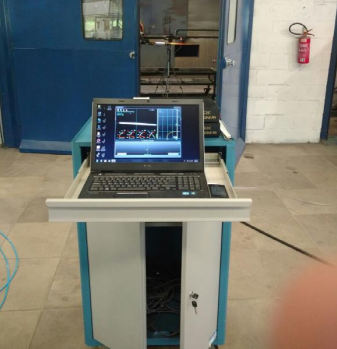
\includegraphics[width=1\columnwidth]{method/figs/adequacao/adequacao1.png}
    \caption{Monitoramento da temperatura e velocidade da chama de aspersão (janeiro/2016).}
    \label{fig:adequacao1}
\end{figure}

As vazões e pressões dos gases de combustão do processo durante o teste de
operação da pistola em longas distâncias é regulado no console do equipamento
enquanto que o resultado da medição dos parâmetros de chama durante o teste é
visualizado no notebook com o software do Accura Spray.

A montagem e realização dos testes de operação com variação da altura de
aspersão são realizadas juntamente com o ajuste do equipamento Accura Spray na
condição de operação mais baixa possível, próximo a 0 m. Após o posicionamento
do robô e do accura spray é realizado a avaliação inicial da chama para a
altura de 0 m. Da mesma forma anterior, os parâmetros de chama medidos nessas
condições são visualizados na interface do accura spray.

Para a execução dos testes utilizando o manipulador com a pistola em posições
mais elevadas foi realizada a instalação de uma bomba para evitar a queda da
pressão de água de refrigeração da pistola. Após o posicionamento, teve de ser
realizada uma aferição visual do paralelismo do cabeçote com a chama de
aspersão, para evitar desvios na medição. Na ultima etapa desse teste foi
realizada aspersão com o manipular posicionado em 4 m de altura, juntamente com
instalação do cabeçote do Accura Spray conforme Fig.~\ref{fig:adequacao2}.

A Tabela~\ref{tab:hvof_tab5} apresenta os resultados registrados pelo sensor de
chama.

\begin{table}[]
\centering
\caption{Valores registrados pelo sensor de chama Accura spray no teste de
metalização em diferentes alturas do braço robótico.}
\label{tab:hvof_tab5}
\begin{tabular}{lll}
\hline
\begin{tabular}[c]{@{}l@{}}Altura\\ de aspersão (m)\end{tabular} & \begin{tabular}[c]{@{}l@{}}Velocidade\\ da chama (m/s)\end{tabular} & \begin{tabular}[c]{@{}l@{}}Temperatura\\ da chama (°C)\end{tabular} \\ \hline
\multicolumn{1}{|l|}{0}                                          & \multicolumn{1}{l|}{608}                                            & \multicolumn{1}{l|}{1592}                                           \\ \hline
\multicolumn{1}{|l|}{1.3}                                        & \multicolumn{1}{l|}{682}                                            & \multicolumn{1}{l|}{1553}                                           \\ \hline
\multicolumn{1}{|l|}{2.6}                                        & \multicolumn{1}{l|}{630}                                            & \multicolumn{1}{l|}{1632}                                           \\ \hline
\multicolumn{1}{|l|}{4}                                          & \multicolumn{1}{l|}{588}                                            & \multicolumn{1}{l|}{1590}                                           \\ \hline
\end{tabular}
\end{table}

\begin{figure}
	\centering
	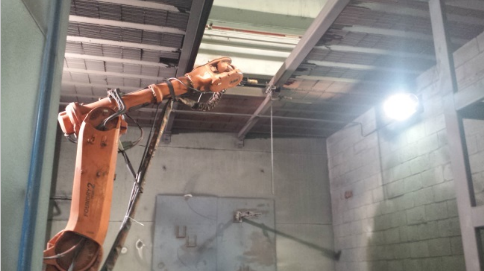
\includegraphics[width=1\columnwidth]{method/figs/adequacao/adequacao2.png}
    \caption{Posicionamento do robô e programação do movimentador, posicionamento dos corpos de prova e do Accura Spray para aplicação em 4  metros (janeiro/2016).}
    \label{fig:adequacao2}
\end{figure}

O uso de combustível GLP foi investigado no processo de aspersão a partir de
corpos de prova metálicos. A análise de desempenho é medida por ensaios de
adesão, metalografia e microdureza. Os elementos do teste são: pó de carboneto
de tungstênio com matriz de cobalto e cromo, GLP e oxigênio como gases da combustão, nitrogênio para
arraste do pó, ar comprimido e água para refrigeração da pistola, e uma pistola
de metalização Diamond Jet modelo DJ2700 (sulzer com refrigeração híbrida). O
equipamento de metalização utilizado para realização do processo de aspersão
produz a chama para a fusão do pó metálico a partir da combustão do
propano. Neste estudo foram realizados testes prévios utilizando-se o GLP como
gás combustível a fim de encontrar os parâmetros ideais de funcionamento do
equipamento para a deposição de um revestimento sem perda de características
técnicas. 

Os resultados foram comparados com os critérios pré-definidos pelo fabricante
da matéria prima e outros testes utilizando propano como
combustível. Nessa perspectiva, não houve perda de características técnicas do
revestimento a partir do uso do GLP como combustível. A importância desse teste
está relacionada com a facilidade de fornecimento de GLP em relação ao propano,
pois como se trata de uma solução abrangente e as usinas hidrelétricas
situam-se muitas vezes em locais ermos com baixas opções de fornecimento de
insumos. A distinção básica entre o GLP e o propano trata-se de que o GLP é uma
mistura de propano e butano e, além disso, possui custo reduzido (~ R\$ 5,00/kg)
de fornecimento em relação ao propano (~R\$16,00/kg). Deve ser feito uma
observação para utilização do GLP em locais frios, pois a sua temperatura de
vaporização é mais elevada tornando a vazão de fornecimento instável. Esse
problema não se aplica, porém, para a região de Porto Velho – RO onde se
encontra a UHE Jirau. A Fig.~\ref{fig:adequacao3} apresenta uma imagem do
ensaio de metalografia realizado em amostras de revestimento aspergido com GLP juntamente
com os resultados dos ensaios citados anteriormente.

\begin{figure}
	\centering
	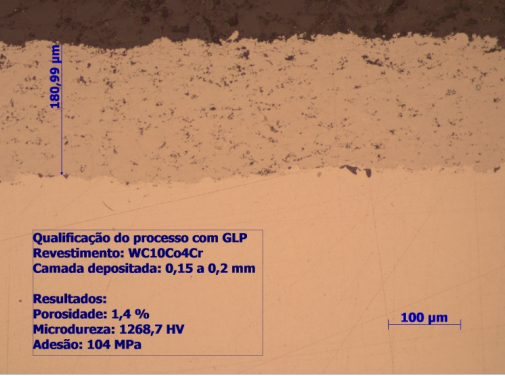
\includegraphics[width=1\columnwidth]{method/figs/adequacao/adequacao3.png}
    \caption{Propriedades do revestimento de Carboneto de Tungstênio-Cobalto-Cromo via HVOF com combustível GLP.}
    \label{fig:adequacao3}
\end{figure}

\subsubsection{Reaplicação de revestimento sobre superfície desgastada}
Com o intuito de testar a metalização sobre o revestimento já desgastado da pá
e o seu desempenho quanto à adesão, um teste de aplicação sobre revestimento
desgastado foi conduzido. Foi utilizada a seguinte metodologia: jateamento dos
corpos de prova metálicos; aplicação de 0.1 mm de camada de WC; medição da
rugosidade; polimento do revestimento com lixa 200; medição da rugosidade; jateamento
sobre superfície revestida e polida; medição de rugosidade; metalização sobre
revestimento polido e jateado; execução dos ensaios de adesão e dobramento e
metalografia.

Para avaliação do desempenho de aspersão térmica aplicada sobre revestimento
remanescente de uma peça, foi necessário realizar um teste de revestimento com
desgaste, jateamento sobre o revestimento, e a avaliação da adesão do conjunto.
Após as medições, foi realizado um polimento da superfície com lixa 300 para
desgastar o revestimento de carboneto de Tungstênio. No momento em que a
superfície ficou com desgaste na qual a rugosidade Ra ficasse abaixo de 1.0
micron, o polimento foi cessado e a medição de espessura foi realizada para
garantir que ainda havia camada de revestimento duro para posterior jateamento
e aspersão. 

Os testes de dobramento são realizados de forma comparativa com a
superfície somente jateado, sem revestimento prévio. No ensaio de dobramento,
avaliou-se que há formação de trincas na superfície do revestimento a partir
do dobramento em 90° de uma chapa com espessura de 4.0 mm em um mandril com
diâmetro de 16 mm. Comparativamente com a amostra sem revestimento prévio
poucas trincas apareceram e não houve destacamento do revestimento, com exceção
das bordas, porém em nível aceitável. Para o teste de adesão conforme a norma
ASTM C633 é considerado um resultado como garantia de adesão apropriada uma
tensão mínima de destacamento de 70 Mpa. O resultado do ensaio de adesão
atendeu a esse critério, com o rompimento se dando na cola utilizada para
realizar o ensaio.

\subsubsection{Seleção dos revestimentos}

A aplicação com uso de Accura Spray para ajuste de parâmetros é
realizado para avaliar as modificações de vazão de gases no ajuste da
chama de aspersão. Para cada configuração de mistura de gases é registrado a
velocidade e temperatura da partícula aspergida a fim de se obter o melhor
parâmetro de aspersão, melhorando o rendimento e as propriedades do
revestimento. Foram utilizados 5 parâmetros de aspersão com o material de
Carboneto de Tungstênio-Cobalto Cromo com tamanho de grão entre 11 microns e 45 microns
(WCCoCr). O parâmetro que forneceu revestimento com menor nível de porosidade
foi replicado para aspergir material com Carboneto de Tungstênio-Cobalto Cromo
com tamanho de grão entre 15 microns e 45 microns (WS11) e material com
Carboneto de Tungstênio-Niquel Cromo (WCNi). Para todos os materiais foram
realizados ensaios para avaliação de resistência à corrosão, além do material
em aço inoxidável AISI 410 sem revestimento.

A aspersão com uma pistola de coating do tipo DJ2700 forneceu a
melhor característica de chama com os seguintes parâmetros: vazão de 72 L/min a
100 Psi de Combustível; vazão de 260 L/min a 150 Psi de Oxigênio; vazão de 340
L/min a 100 Psi de Ar comprimido; taxa de alimentação de pó de 40 g/min;
distância de trabalho de 230 mm; ângulo de aspersão de $90\circ$; velocidade de
deslocamento da pistola de 500 mm/s; velocidade de chama medida de 700 m/s; e
temperatura de chama medida de 1780 °C via Accura Spray. Os testes destrutivos
em corpos de prova WCCoCr e WCNi são realizados nestas condições.

As técnicas empregadas no estudo de resistência a corrosão dos sistemas (aço
inox AISI 410 recoberto por HVOF por camadas a base de WC) são: registro do
potencial do circuito aberto (OCP); e curvas de polarização eletroquímica. 

O potencial de circuito aberto é uma das variáveis que pode indicar a
suscetibilidade à corrosão. Em geral, quanto menor esse valor, maior será à
corrosão do sistema em estudo. Há uma tendência de que o material corroa mais no
sistema que apresente potenciais mais baixos em relação ao que apresente
potenciais mais altos. O potencial de circuito aberto (OCP) é medido por 60
minutos e, em seguida, é realizado ensaio de polarização potenciodinâmica
por um potenciostato/galvanostato, e uma célula eletroquímica,
onde a qual é disposta em uma gaiola de Faraday para diminuir as interferências
elétro-magnéticas externas. Este OCP pode ser observado também nas curvas
de polarização quando a corrente tende a zero.

A curva de polarização eletroquímica é outra análise que permite avaliar o
comportamento à corrosão de um determinado sistema metal-meio. Nessa técnica,
pode-se modificar o potencial de repouso (potencial de circuito aberto) para
valores mais positivos de potencial acelerando o processo corrosivo. A taxa de
corrosão esperada será proporcional à densidade de corrente registrada. Esse
ensaio permite determinar o potencial de pite, o qual será o potencial onde se
observa um aumento brusco de corrente.

Para todos os ensaios foi utilizada uma célula convencional de três eletrodos,
com eletrodo de calomelano saturado (ECS) como eletrodo de referência e eletrodo
de platina como contra eletrodo. As medidas foram realizadas em solução aquosa
de 3,5\% de NaCl em peso, não agitada, naturalmente aerado e à temperatura
ambiente. O potencial de circuito aberto (OCP) foi monitorado durante a primeira
hora de imersão no eletrólito antes do ensaio de polarização. O intervalo de
varredura foi de -100 mV abaixo do potencial de circuito aberto até 300 mV acima
do OCP, com uma velocidade de varredura de 1 mV/s.

Na Fig.~\ref{fig:adequacao4}, (A) mostra as curvas de potencial de circuito
aberto das amostras que sofreram variações nos parâmetros de deposição, com o
intuito de diminuir a porosidade dos revestimentos. Em todos os sistemas são
observados uma redução nqo potencial de circuito aberto com o decorrer do tempo,
podendo indicar um aumento de agressividade da solução presente nas irregularidades das camadas revestidas.
Não é possível observar diferenças significantes entre as curvas OCP, no
entanto, o sistema 4 apresentou potenciais mais ativos de corrosão comparado com
os demais sistemas, possivelmente pelo alto nível de porosidade presentes no
revestimento.

\begin{figure}
	\centering
	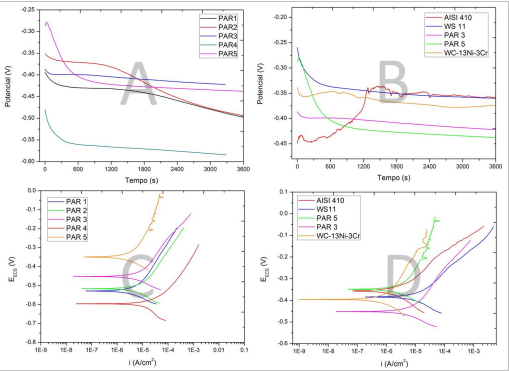
\includegraphics[width=1\columnwidth]{method/figs/adequacao/adequacao4.png}
    \caption{(A): Potencial de Circuito Aberto, com variação de parâmetros de
    aspersão térmica dos revestimentos de WC-10Co-4Cr com granulometria do pó
    11/45; (B) Potencial de Circuito Aberto de diferentes sistemas comparando
    com o substrato Jateado; (C) Ensaio de Polarização com variação de
    parâmetros dos revestimentos de WC-10Co-4Cr com granulometria do pó 11/45;
    (D) Ensaio de polarização dos diferentes sistemas comparando com o
    substrato jateado.}
    \label{fig:adequacao4}
\end{figure}

Para as curvas de OCP apresentadas na Fig.~\ref{fig:adequacao4} (B), foi
selecionado os dois revestimentos com menores porosidades nas medições anteriores assim como o
substrato, o WS 11 o qual foi utilizado pó com granulometria diferente e o WCNi.

Conforme já comentado, os sistemas revestidos sofreram redução ao longo do tempo
pela provável modificação da solução no interior dos poros, ao contrário do
comportamento do substrato, que por ser maciço, não apresenta poros. Neste caso
observa-se um aumento do potencial de corrosão com o tempo, indicando redução no
processo corrosivo, possivelmente devido ao espessamento do filme protetor do
óxido de cromo.

Na Fig.~\ref{fig:adequacao4} (C), são apresentados os ensaios de polarização
eletroquímica da variação de alguns parâmetros operacionais. Nota-se que os
revestimentos com menores porosidades apresentam potencial de circuito aberto
(quando a curva tende a zero) mais elevado (menos negativos) indicando menor
taxa de corrosão. Além disso, à medida que a porosidade é reduzida, as curvas de
polarização tendem a se deslocar a esquerda, no sentido das menores correntes,
resultando em menores taxas de corrosão.

Na Fig.~\ref{fig:adequacao4} (D), são apresentadas as curvas de polarização dos
sistemas que tiveram menores porosidades e melhores desempenhos na
Fig.~\ref{fig:adequacao4} (C), o substrato de aço inoxidável AISI 410 jateado, a
amostra WS 11 utilizando um pó com granulometria de 15/45 e a amostra WCNi com
matriz de níquel. Analisando a Fig.~\ref{fig:adequacao4} (D), pode-se dizer
preliminarmente que os sistemas que apresentaram melhor desempenho frente a
corrosão, protegendo efetivamente o substrato, são os sistemas 5 e o WCNi. Esse
resultado é fruto de apenas uma técnica, necessitando de confirmação com outros
tipos de ensaios que considerem tempos mais longos de exposição das amostras ao
meio. Como, por exemplo, ensaio de imersão ou impedância eletroquímica.

Pode-se concluir que os teores de porosidade crescentes pioram o desempenho da
camada em proteger o substrato contra corrosão. Entre as camadas estudadas, as
que apresentaram efetiva proteção ao substrato foram os sistemas 5 e WCNi. A
presença de níquel no revestimento demonstra ser promissor em relação à proteção
do substrato à corrosão.